
%%%%%%%%%%%%%%%%%
% Configuration %
%%%%%%%%%%%%%%%%%

\documentclass[12pt, a4paper, twocolumn]{article}
\usepackage{xurl}

\usepackage{abstract}
\renewcommand{\abstractnamefont}{\normalfont\bfseries}
\renewcommand{\abstracttextfont}{\normalfont\small\itshape}
\usepackage{lipsum}
\usepackage[affil-it]{authblk}
\usepackage{natbib}
\usepackage{graphicx}% http://ctan.org/pkg/graphicx


%%%%%%%%%%%%%%
% References %
%%%%%%%%%%%%%%

% If changing the name of the bib file, change \bibliography{test} at the bottom

\title{\textbf{Decentralized growth coin: designing a low volatility investment cryptocurrency protocol}}

\author[1]{Pavel Krolevets}
\affil[1]{Department of Computer Science and Engineering, Shanghai Jiao Tong University, China}
\affil[ ]{pavelkrolevets@sjtu.edu.cn}

\newcommand{\abstractText}{\noindent
Nowadays cryptocurrency becoming widespread and blockchain technology is taken seriously by global banks and community. There are significant variety of cryptocerrency assests have appeared after success of Bitcoin and Ethereum. Stable coins like USDT ans Dai provided so long anticipated fiat money replacements in the cryptocurrency. However, there rapidly changing financial landscape demands for a new type of blockchain transferable means which will play a role of low risk investments, filling the gap between high volatility original cryptocurrency and stablecoins. 
In this paper we making an attempt to bridge computer science and economics, fostering transfer of expertise. The proposal of this work lies within the uncomfortable middle ground between money definition, cryptographic algorithms, game theory, and unfamiliar paradigm shifts. 

As the result, we propose another kind of decentralized cryptocurrency protocol - low volatility growth coin which can be used as a safe investment and a direct competitor for bank deposits or bond investments, accompanied with stablecoin and high volatility asset.
}


% Any configuration that should be done before the end of the preamble:
\usepackage{hyperref}
\hypersetup{colorlinks=true, urlcolor=blue, linkcolor=blue, citecolor=blue}

\begin{document}

%%%%%%%%%%%%
% Abstract %
%%%%%%%%%%%%

\twocolumn[
  \begin{@twocolumnfalse}
    \maketitle
    \begin{abstract}
      \abstractText
      \newline
      \newline
    \end{abstract}
  \end{@twocolumnfalse}]

%%%%%%%%%%%
% Article %
%%%%%%%%%%%

\section{Introduction}
Blockchain technology  is changing the landscape of financial industry by providing new possibilities of automation, security, and trust. Success of the first cryptocurrency Bitcoin proved that a long term cryptographical dream can materialize and be a mean of decentralized cryptocurrency. A successor, Ethereum paltform went further and provided a new type of decentralized computaton and storage - blockchain based virtual computational machine which can be used to execute the code in the decentralized manner. An impact to financial industry is unarguably significant. Financial industry received new ways of processes automation and decentralization.
  
We are not going to dig deep into the history of cryptocurrecncy and blockchain as we assume a reader already familiar with it. For those who want to refresh their memory or learn about the history of digital cash protocols and final appear of cryptocurrency can refer to \cite{MasteringBitcoin, MasteringEthereum}.

Any financial system cannot exist without stable low volatility assets. Very high volatility of cryptocurrency is a one of the main problems preventing it of wide use. As a attempt to solve this problem a price stabilized cryptocurrency was introduced which is pegged to the price of a fiat currency, creating a layer on top of the existing monetary system.

Pegging cryptocurrency to fiat currency inherently has problems. First, it affected from the decisions of the Central bank and, therefore, cannot be claimed absolutely decentralized despite of the underlying protocol of the stablecoin. Second, it can affect effectiveness of the Central bank monetary policies if the stablecoin accumulates significant capitalization. In this case it can be subject of the additional regulation. 



This paper is organized as follows. In Section II, we review price stabilization mechanisms. In Section III, we describe a design of a non-collateralized low-volatility growth token protocol. In conclusion, we summarize the meaning of this paper and state challenges for the future. This is the first survey ofstablecoins to the best of our knowledge. 

\section{Preliminary}

\subsection{Stablecoins}

\textit{Stablecoin}  - is a blockchain cryptocurrency with a price stabilization mechanism. Usually its pegged to an exchange rate of a real asset like USD, but there are attempts to peg the price to gold \cite{digix}

The first of its kind stable crypto-asset pegged to USD fiat currency (Tether) was introduced in 2012 by J.R. Willett \cite{tether}. Its main idea was to create a pool of real assets and issue an equal amount of cryptocurrency tokens with the promise to exchange this tokens to real assets at any time. The demand and anticipation for such an asset was very high and it had a quiet a success despite the fact that it uses collateral as a price stabilization mechanism and, therefore, centralized. 

As an attempt to create the first truly decentralized stable criptocurrency in 2014 Maker DAO team introduced Dai (formerly called eDollar) stable coin pegged to USD \cite{dai}. This system is built on a set of smart contracts and keeps a soft peg to USD real currency by supply/demand forces coming from Dai creators who is basically margin borrowers and a collateral is their cryptoassets. Maker Team also introduced a decentralized way of creating an oracle to determine current cryptoasset exchange rate to keep overall system margin above set level. 

Dai protocol approach suffers from a margin call problem in case of severe asset price depreciation or speculative economic attack. The design of the protocol allows a decline of the underlying collateral (Ethereum cryptocurrency) to the level not lower than 80 percent. In this case a global margin call is initiated and all operations are halt till the decentralized owners of the system make an action. This theoretically minimizes the risk of system shutdown and loss of the collateral, but it has never been tested in real environment and still raises some questions. Another problem which Dai protocol suffers is overcollaterization. 

\subsection{Price stabilization mechanisms}
At the top level we can classify price stabilization mechanisms to collateralized and non-collaterized. In the former there is no real asset exists to link to value of the token. 
Also its possible to classify non-collaterized price stabilization mechanism to protocol layer and application layer  \cite{DBLP:journals/corr/abs-1906-06037}. 

\subsubsection{Tokenization of collateral (application layer)}

 \textit{A. Direct collateriziation} mechanism is, probably, one of easier to understand. It is well studied and often used in real world applications. The main idea is to provide a frictionless means to exchange of some reprezenation of an asset (token) to the asset itself. A collateral can be any real asset, like currency, gold, oil, etc. This is used by some degree of success by Tether stablecoin \cite{tether}. 

However, this approach has a significant amount of detriments:
\begin{itemize}
\item require some degree of centralization, a trusted third party is needed to manage the funds
\item frictionless market transactions is impossible to achieve
\item high degree of counterparty risk
\item low protection against economic speculative attack
\end{itemize}

\textit{B. Proxy collateriziation} is a type of collaterized mechanism, but instead tokens are linked to the price of another cryptocurrency or a backet of assets. This can help mitigate some of the detriments of direct collaterization and allow more decentralization as counterparty risk can be eliminated, but it suffers from different types of risks:
 \begin{itemize}
\item oracle problem. The trusted mechains needed to determine the price of a proxy asset. This is difficult to implement because of limitations on blockchain interaction with the real world. 
\item difficult to maintain a peg to a proxy with high volatility like Bitcoin
\item risk of undercollaterization
\end{itemize}

\textit{C. Self-collateriziation}. This is a form of proxy collaterization, but the stabilized token is backed by the underlying cryptocurrency. Exhibits mostly similar problems as proxy collaterization.

\textit{D. Interest rate mechanism}. In this approach  interest rate on loans and deposits is used to control the price of a token. Demand for tokens comes from loans which is created from proxy cryptocurrency. Users lock proxy cryptocurrency to mint new stabilized tokens. They are free to use these tokens while not loosing the  ownership of original proxy token. Basically they create a collaterized loan. The interest they pay for this loan is \textit{stability fee}, which is controlled by the governance of the system. The higher a stability fee the less loans are created, decreasing the supply of stabilized tokens. When there is a need to decrease the supply, interest rates on loans increased and  less tokens are supplied. When users want to take their collateral back, they return stabilized coin and pay the stability fee. An oracle is used to determine equality of amount of stabilized tokens in the system to the value of the collateral. Margin call is used to  \textit{Maker Dai} is the first successful project which uses this stabilization mechanism \cite{dai}. 
Its worth to mention, that in decentralized settings its difficult to implement undercollaterized loans when future income can be taken as a collateral. In \cite{1905.11905} authors argue that its impossible to implement in permisionless cryptocurrency because of general anonymity of identities and vulnerability for Sybil attacks.

Problems which this approach suffers from:
\begin{itemize}
\item oracle problem. To determine the value of the collateral an oracle is required, which makes it susceptible to an attack on oracle or data providers. 
\item margin call as mechanism to control the risk of undercollaterization.
\item generally a need in overcollaterization for stability of the system.
\end{itemize}

\subsubsection{Open market interventions (application layer)}
In this technique a direct market interventions are used to adjust the price of a token. When demand increases new tokens are provided in exchange for the pegged asset and the reserve is created. On the other hand, tokens are bought back from the market using a reserve to affect token price. This approach is naturally centralized to some degree as there should be a central authority to stabilize the price of the token. This approach is mimicking the Central bank operations when it sells or buy treasuries on the market to increase/decrease of the money supply and based on . 
Seigniorage shares \cite{SeigniorageShares} approach falls to this section, because it  when supply expands, shareholders of the system receive new stablecoins, otherwise there are new shares issued, which are paid back when there is an expansion. Basecoin \cite{basis} project is an example of this type of the protocol.

\subsubsection{Block rewards and transaction fees (protocol layer)}

It is also worth mentioning that economical principles of asset price appreciation are embedded to Bitcoin  \cite{nakamoto2012bitcoin}  and Ethereum  \cite{buterin2014ethereum}  protocols through increase in computational complexity in Proof-of-Work consensus algorithm and consequent decrease in supply. For example, PoW consensus algorithm adjusts difficulty of a block creation based on the speed of successful mining, keeping supply limited depends on speed of mining . However, these protocols don't take in consideration market demand of the underlying token, that can lead to high volatility of the token value. Some research attempts exist to solve this problem and implement techniques to stabilize underlying cryptocurrency exchange rate \cite{1801.06771}.

\begin{figure*}
  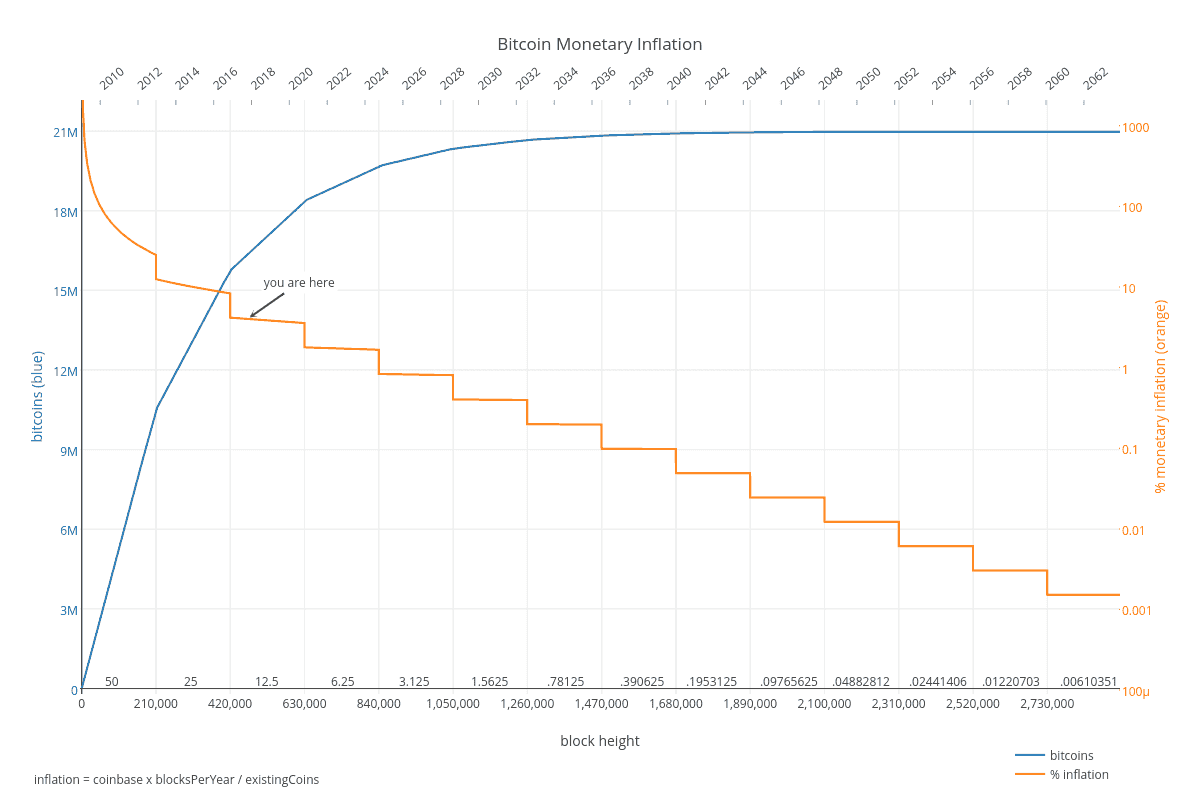
\includegraphics[width=\textwidth,height=4cm]{Bitcoin_Monetary_Inflation.png}
  \caption{Bitcoin inelastic sypply (source: http://bashco.github.io/)}
\end{figure*}

\subsection{Motivation}
Financial system cannot function properly without low volatility low risk assets. They play a major role in risk management and stabilization of the system. In newly formed alternate world of cryptocurrency finance there is a significant lag between types of crypto assets and real world assets exist. Such a constantly growing token would form a building block for the crypto financial system. Stable coins, which pegged to a real fiat currency, appeared just recently. But there are no low volatility, stable growng token present. In this paper we aim to design such a protocol which can be used later for more sophisticated applications.

\subsection{Related work}

Maker team \cite{dai} made an attempt to create a non-collaterelized stablecoin system pegged to US dollar using interest rate price stabilization mechanism. In their protocol design they created a kind of growth (MKR) token which value appreciates based on inflow from fees gathered from leveraged creation of a stablecoin Dai.

Exeum is another attempt to create a stablecoin system..... \cite{1808.03482}
 
 \section{Protocol design}
In the creation of low volatility growth coin we need to be very clear about what we are trying to achieve and the role it will play in the crypto-financial system. Stablecoins play a significant role in stabilizing cryptocurrency market, but there is no value appreciation mechanisms embedded to use it as a safe investment vehicle. Therefore we can define goal we are trying to achieve:
\begin{enumerate}
\item Continuous value appreciation based on pure market forces, not market manipulation.
\item Low price volatility. Comparable to other stablecoin protocols.
\item Stability of the system in the case of catastrophic cryptocurrency market moves.
\item Robustness of the system to all types of adversarial attacks: security, governance  and speculative attacks.
\item Decentralization of the protocol.
\end{enumerate}
 
Lets define market forces which can drive value appreciation of the token. There are several types of market forces which can drive value appreciation of the token:

\begin{itemize}
\item \textit{Dynamic and constant decrease in supply} 
 
In this case we should dynamically keep supply of tokens less than demand, but control it adequate to market environment. This approach doesn't seem sustainable as its not clear how to drive value appreciation in the case of constant low demand. Moreover, its difficult to implement price stabilization mechanisms and unclear which role this token will play.
\item \textit{Open market interventions}

This approach doesn't seems sustainable also, as it artificially affect the price of the token and requires some authority to sell and buy tokens on the open market. Moreover, there is a limit in which market price can be affected which depends on the reserve amount devoted for market interventions.
\item \textit{Interest rate on borrowing}

This approach based on the principle in the real economy when the Central bank lend/borrow money effectively increasing and decreasing supply. Also, there are speculators, who use leverage to speculate on the price of the asset and ready to pay interest on the leverage they create. In this case, the value appreciation of the token can have a more sustainable source, but other mechanisms like market interventions can be used for stabilization of the token.
\end{itemize}

As we postulate that the main driving force in the cryptocerrency finance is interest rate on borrowing for marging speculating, as there is no Central bank present and no inflation is observed. Some form analogues to the Central bank can be implemented through decentralized governance system. This type of monetary cryptocurrency system can be called private comparing to the existing Central bank monetary system.
As the Central bank target inflation by manipulating money supply through the interest rate and direct interventions with interest bearing instruments, the private system can take this principle as a basis and adjust for decentralized governance settings, effectively producing interest bearing token and a relatively stable pegged token.

We are going to refer to Maker DAO project \cite{dai} where two types of tokens are used, a pegged to USD token Dai and a governance share token MKR. In our case the most interest is lies in the governance token, which by design should appreciated in value based on fees are taken from the system for taking the risk of global margin call. \textit{\textbf{In contrast of this approach we are going to focus on both - the governance token and the pegged token and try to link it to the modern monetary theory}} \cite{randallwray2012}. 

Main parts of the system from the high level perspective:

\begin{itemize}
\item \textit{Decentralized lending mechanism} (similar to Maker Dao \citep{dai}). Enables third parties to borrow funds from the system using native token.
\item \textit{Decentralized governance subsystem}. Should be an effective voting system in place to get votes  from the main stakeholders. Will represent a decentralized central bank system.
The governance system based on the voting mechanism of the main stakeholders. At the end of each epoch token holders will have a right to vote on the main interest rate set in the system. Because,  the growth token is freely traded on the market, to get a vote right they should hold it at least a full epoch. 
\item \textit{Oracle subsystem} to gather information about pegged currency exchange rate, CPI and other required indicators.
\item \textit{Price/volatility stabilization subsystem} for the pegged and growing tokens.
\item \textit{Reserve subsystem and safety mechanisms}.
The reserve system represents the collateral and acts as a guarantor for the main users and stakeholders. 
\item \textit{Security monitoring/enforcement subsystem}.
\end{itemize}
 
\textit{The core} mechanism of the system is the global interest rate on lending to other cryptocurrency market participants, similar approach is taken by Maker project, but with novel contributions discussed further.

We can distinguish three main stakeholders in the system: users interested to invest in low volatility/risk cryptocurrency asset and get passive return; main stakeholders of the system responsible for the governance; users of stabilized cryptocurrency pegged to real-world currency; borrowers from the system (usually active traders).

The system has three main types of tokens freely circulating on the market:
\begin{itemize}
\item Bond-like token, which value appreciates constantly with low volatility.
\item Pegged to real currency token (USD).
\item System utility token.
\end{itemize}

System description:

Borrowers from the system generates new pegged to real-world currency tokens by creating a collaterized debt position by sending their cryptocurrency (Bitcoin, Ethereum, etc.) to a smart contract. The smart contract locks assets as a collateral and generates pegged tokens in the amount equals to 0.5 of the collateral value to keep a leverage at 1.5 level. To close this borrowing position and receive back collateral borrowers should send created tokens back to the smart contract.

The borrowers pay a fee determined by the global interest rate, which is set through the decentralized governance system. This will affect the demand to our target growth token, which represent an alternative to treasury bonds, but is perpetual, accumulates interest in the form of value appreciation. Users of the system will buy this growth token in the open market creating a reserve which will be carefully monitored by the stakeholders and stabilization mechanisms. High level system design and economics is presented in figure 2.








\begin{figure*}
  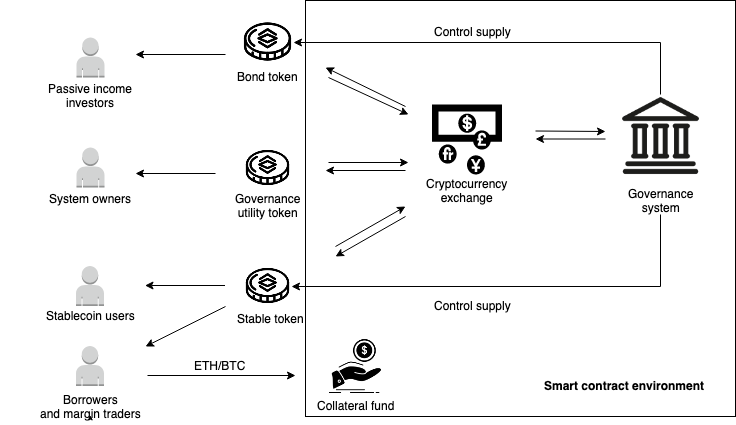
\includegraphics[width=\textwidth,height=7cm]{GeneralSchema.png}
  \caption{General schema reflecting participants: passive income investors)}
\end{figure*}

 \subsection{Decentralized governance system}
 
 
  \section{Collected reusable garbage}
 
Three functions of money:
 \begin{itemize}
\item Unit-of-Account
\item Medium-of-Exchange
\item Store-of-Value
\end{itemize}



market forces which will affect this type of growing stablecoin.
 
As a result of the protocol we are going to create thee types of tokens: stablecoin pegged to USD, low volatility growth token based on interest rates in the system, and a share token. 
  


%%%%%%%%%%%%%%
% References %
%%%%%%%%%%%%%%
\bibliographystyle{plain}
\bibliography{ref}

\end{document}
